\chapter{Archive}
\section{LC 0258 - Add Digits (Digit Root)}
Given an integer {\colorbox{CodeBackground}{\lstinline|num|}}, repeatedly add all its digits until the result has only one digit, and return it.\\

Examples:
\begin{itemize}
\item {\colorbox{CodeBackground}{\lstinline|num = 38 --> 2|}}
\begin{lstlisting}
38 --> 3 + 8 --> 11
11 --> 1 + 1 --> 2 
\end{lstlisting}
\item {\colorbox{CodeBackground}{\lstinline|num = 0 --> 0|}}
\end{itemize}

\subsection*{Solution 1 - Brute Force (Iterative)}\label{solution:lc0258_simulation_iterative}
\begin{lstlisting}
int addDigits(int num) {
  while (num >= 10) {
    int sum = 0;
    while (num > 0) {
      sum += num % 10;
      num /= 10;
    }
    num = sum;
  }
  return num;
}
\end{lstlisting}

\subsection*{Solution - Brute Force (Recursion)}\label{solution:lc0258_simulation_recursion}
\begin{lstlisting}
int addDigits(int num) {
  if (num < 10) { return num; }
  int sum = 0;
  while (num > 0) {
    sum += num % 10;
    num /= 10;
  }
  return addDigits(sum);
}
\end{lstlisting}

\subsection*{Solution 2 - Mathematical Formula}\label{solution:lc0258_mathematical_formula}
\begin{lstlisting}
int addDigits(int num) {
  if (num == 0) { return 0; }
  return num % 9 == 0 ? 9 : num % 9;
}
\end{lstlisting}

\subsection*{Solution 3 - Mathematical Formula, Optimized}\label{solution:lc0258_mathematical_formula_optimized}
\begin{lstlisting}
int addDigits(int num) {
  if (num == 0) { return 0; }
  return 1 + (num - 1) % 9;
}
\end{lstlisting}

\section{LC 0529 - Minesweeper}
Let's play the minesweeper game!\\

You are given an {\colorbox{CodeBackground}{\lstinline|m x n|}} char matrix {\colorbox{CodeBackground}{\lstinline|board|}} representing the game board where:
\begin{itemize}
\item {\colorbox{CodeBackground}{\lstinline|'M'|}} represents an \ul{unrevealed mine};
\item {\colorbox{CodeBackground}{\lstinline|'E'|}} represents an \ul{unrevealed empty square};
\item {\colorbox{CodeBackground}{\lstinline|'B'|}} represents \ul{a revealed blank square that has no adjacent mines} (i.e., \ul{above}, \ul{below}, \ul{left}, \ul{right}, and \ul{all {\colorbox{CodeBackground}{\lstinline|4|}} diagonals)};
\item Digit ({\colorbox{CodeBackground}{\lstinline|'1'|}} to {\colorbox{CodeBackground}{\lstinline|'8'|}}) represents \ul{how many mines are adjacent to this revealed square};
\item {\colorbox{CodeBackground}{\lstinline|'X'|}} represents a \ul{revealed mine}.
\end{itemize}

You are also given an integer array {\colorbox{CodeBackground}{\lstinline|click|}} where {\colorbox{CodeBackground}{\lstinline|click = [r, c]|}} represents the \ul{next click position} among all the unrevealed squares ({\colorbox{CodeBackground}{\lstinline|'M'|}} or {\colorbox{CodeBackground}{\lstinline|'E'|}}).\\

Return the board after revealing this position according to the following rules:
\begin{enumerate}
\item If a mine {\colorbox{CodeBackground}{\lstinline|'M'|}} is revealed, then the game is over. You should change it to {\colorbox{CodeBackground}{\lstinline|'X'|}}.
\item If an empty square {\colorbox{CodeBackground}{\lstinline|'E'|}} with no adjacent mines is revealed, then change it to a revealed blank {\colorbox{CodeBackground}{\lstinline|'B'|}} and all of its adjacent unrevealed squares should be revealed recursively.
\item If an empty square {\colorbox{CodeBackground}{\lstinline|'E'|}} with at least one adjacent mine is revealed, then change it to a digit ({\colorbox{CodeBackground}{\lstinline|'1'|}} to {\colorbox{CodeBackground}{\lstinline|'8'|}}) representing the number of adjacent mines.
\item Return the board when no more squares will be revealed.
\end{enumerate}

\begin{itemize}
\item Example 1
\begin{lstlisting}
board = 
[["E","E","E","E","E"],
 ["E","E","M","E","E"],
 ["E","E","E","E","E"],
 ["E","E","E","E","E"]], 
click = [3,0]
-->
[["B","1","E","1","B"],
 ["B","1","M","1","B"],
 ["B","1","1","1","B"],
 ["B","B","B","B","B"]]
\end{lstlisting}
\begin{figure}[H]
\centering
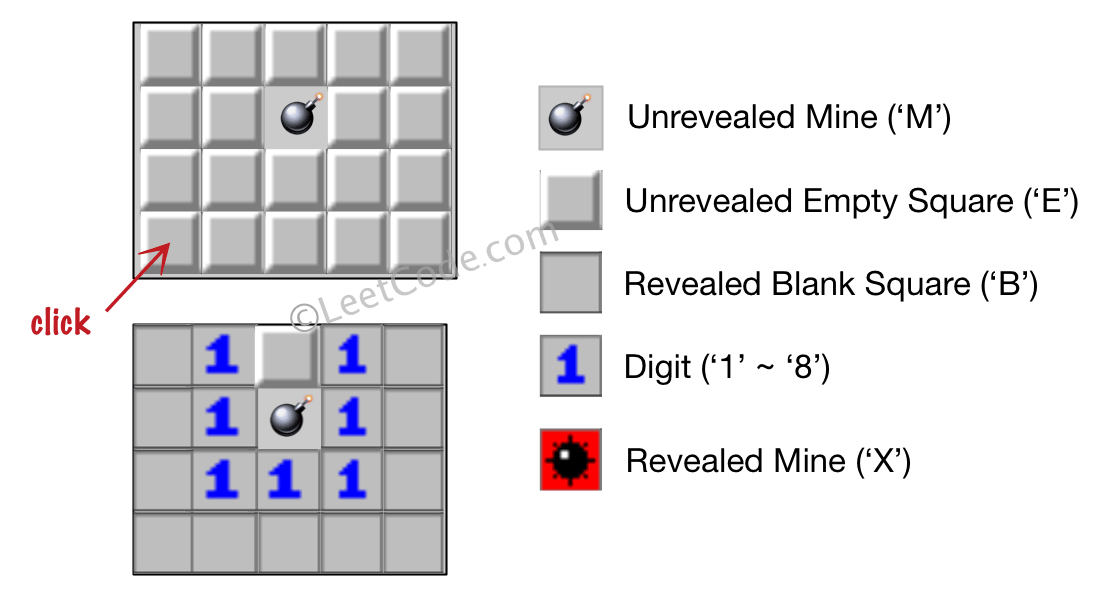
\includegraphics[width=0.4\linewidth]{images/lc0529_eg1}
\label{fig:lc0529eg1}
\end{figure}
\item Example 2
\begin{lstlisting}
board = 
[["B","1","E","1","B"],
 ["B","1","M","1","B"],
 ["B","1","1","1","B"],
 ["B","B","B","B","B"]]
click = [1,2]
-->
[["B","1","E","1","B"],
 ["B","1","X","1","B"],
 ["B","1","1","1","B"],
 ["B","B","B","B","B"]]
\end{lstlisting}
\begin{figure}[H]
\centering
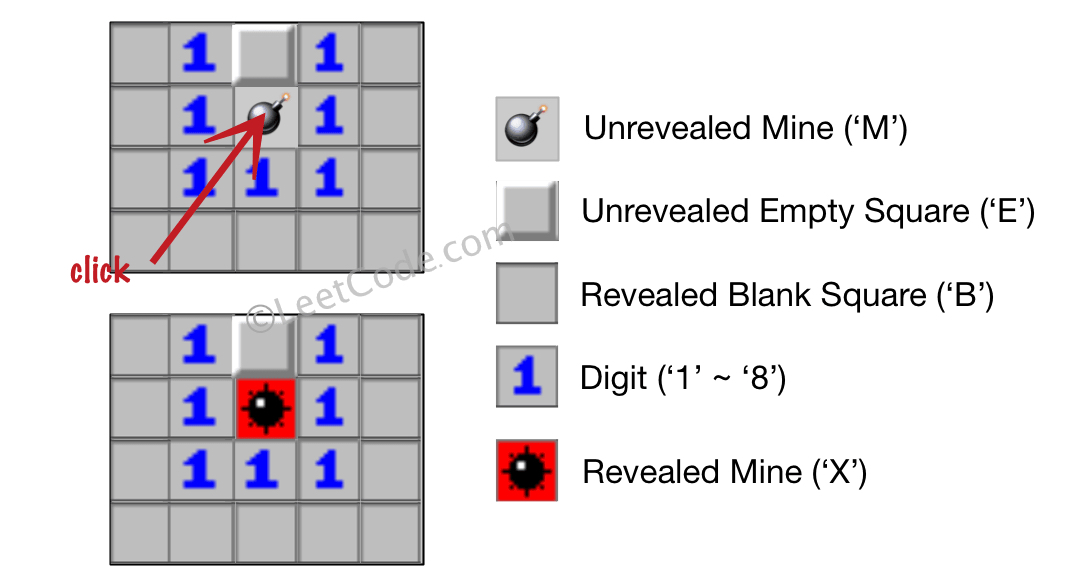
\includegraphics[width=0.4\linewidth]{images/lc0529_eg2}
\label{fig:lc0529eg2}
\end{figure}
\end{itemize}

\subsection*{Solution - DFS}
\begin{lstlisting}
void reveal(std::vector<std::vector<char>>& board, int x, int y) {
	if (x < 0 || x >= board.size() || y < 0 || y >= board[0].size() || board[x][y] != 'E') { return; }
	
	// Directions for the adjacent squares (including diagonals)
	int dirs[8][2] = {{1, 0}, {-1, 0}, {0, 1}, {0, -1}, {1, 1}, {1, -1}, {-1, 1}, {-1, -1}};
	int count = 0;
	
	// First pass to count the adjacent mines
	for (auto& dir : dirs) {
		int newX = x + dir[0], newY = y + dir[1];
		if (newX >= 0 && newX < board.size() && newY >= 0 && newY < board[0].size()) {
			if (board[newX][newY] == 'M') { count++; }
		}
	}
	
	if (count > 0) {
		// If there are adjacent mines, set the count and stop.
		board[x][y] = '0' + count;
	} else {
		// If there are no adjacent mines, reveal all adjacent squares.
		board[x][y] = 'B';
		for (auto& dir : dirs) {
			int newX = x + dir[0], newY = y + dir[1];
			reveal(board, newX, newY);
		}
	}
}

std::vector<std::vector<char>> updateBoard(std::vector<std::vector<char>>& board,
std::vector<int>& click) {
	int x = click[0], y = click[1];
	
	// If the player clicks a mine, game over.
	if (board[x][y] == 'M') {
		board[x][y] = 'X';
	} else {
		// Otherwise, reveal the board based on the click.
		reveal(board, x, y);
	}
	
	return board;
}
\end{lstlisting}

\section{LC 0406 - Queue Reconstruction by Height}
You are given an array of people {\colorbox{CodeBackground}{\lstinline|people|}}, which are the attributes of some people in a queue (not necessarily in order). Each {\colorbox{CodeBackground}{\lstinline|people[i] = [h_i, k_i]|}} represents the {\colorbox{CodeBackground}{\lstinline|i|}}th person of height {\colorbox{CodeBackground}{\lstinline|h_i|}} with exactly {\colorbox{CodeBackground}{\lstinline|k_i|}} other people in front who have a height greater than or equal to {\colorbox{CodeBackground}{\lstinline|h_i|}}.\\

Reconstruct and return the queue that is represented by the input array {\colorbox{CodeBackground}{\lstinline|people|}}. \\

The returned queue should be formatted as an array {\colorbox{CodeBackground}{\lstinline|queue|}}, where {\colorbox{CodeBackground}{\lstinline|queue[j] = [h_j, k_j]|}} is the attributes of the {\colorbox{CodeBackground}{\lstinline|j|}}th person in the {\colorbox{CodeBackground}{\lstinline|queue|}} ({\colorbox{CodeBackground}{\lstinline|queue[0]|}} is the person at the front of the queue).\\

Examples:
\begin{itemize}
\item {\colorbox{CodeBackground}{\lstinline|people = [[7,0],[4,4],[7,1],[5,0],[6,1],[5,2]] --> [[5,0],[7,0],[5,2],[6,1],[4,4],[7,1]]|}}\\
Person {\colorbox{CodeBackground}{\lstinline|0|}} has height {\colorbox{CodeBackground}{\lstinline|5|}} with no other people taller or the same height in front.\\
Person {\colorbox{CodeBackground}{\lstinline|1|}} has height {\colorbox{CodeBackground}{\lstinline|7|}} with no other people taller or the same height in front.\\
Person {\colorbox{CodeBackground}{\lstinline|2|}} has height {\colorbox{CodeBackground}{\lstinline|5|}} with two persons taller or the same height in front, which is person {\colorbox{CodeBackground}{\lstinline|0|}} and {\colorbox{CodeBackground}{\lstinline|1|}}.\\
Person {\colorbox{CodeBackground}{\lstinline|3|}} has height {\colorbox{CodeBackground}{\lstinline|6|}} with one person taller or the same height in front, which is person {\colorbox{CodeBackground}{\lstinline|1|}}.\\
Person {\colorbox{CodeBackground}{\lstinline|4|}} has height {\colorbox{CodeBackground}{\lstinline|4|}} with four people taller or the same height in front, which are people {\colorbox{CodeBackground}{\lstinline|0|}}, {\colorbox{CodeBackground}{\lstinline|1|}}, {\colorbox{CodeBackground}{\lstinline|2|}}, and {\colorbox{CodeBackground}{\lstinline|3|}}.\\
Person {\colorbox{CodeBackground}{\lstinline|5|}} has height {\colorbox{CodeBackground}{\lstinline|7|}} with one person taller or the same height in front, which is person {\colorbox{CodeBackground}{\lstinline|1|}}.\\
Hence {\colorbox{CodeBackground}{\lstinline|[[5,0],[7,0],[5,2],[6,1],[4,4],[7,1]]|}} is the reconstructed queue.
\item {\colorbox{CodeBackground}{\lstinline|people = [[6,0],[5,0],[4,0],[3,2],[2,2],[1,4]] --> [[4,0],[5,0],[2,2],[3,2],[1,4],[6,0]]|}}\\
\end{itemize}

\subsection*{Solution - Greedy}
\begin{lstlisting}
std::vector<std::vector<int>> reconstructQueue(std::vector<std::vector<int>>& people) {
  std::sort(people.begin(), people.end(),
            [](const std::vector<int>& a, const std::vector<int>& b) {
              return a[0] == b[0] ? a[1] < b[1] : a[0] > b[0];
            });

  std::vector<std::vector<int>> queue;
  for (std::vector<int>& person : people) {
    queue.insert(queue.begin() + person[1], person);
  }
  return queue;
}
\end{lstlisting}

\section{LC 2483 - Minimum Penalty for a Shop}\label{lc2483}
\hyperref[sec:prefix_sum]{[Prefix Sum]}\\

You are given the customer visit log of a shop represented by a {\colorbox{CodeBackground}{\lstinline|0|}}-indexed string {\colorbox{CodeBackground}{\lstinline|customers|}} ({\colorbox{CodeBackground}{\lstinline|customers.size() >= 1|}}) consisting only of characters {\colorbox{CodeBackground}{\lstinline|'N'|}} and {\colorbox{CodeBackground}{\lstinline|'Y'|}}:
\begin{itemize}
\item if the {\colorbox{CodeBackground}{\lstinline|i|}}th character is {\colorbox{CodeBackground}{\lstinline|'Y'|}}, it means that customers come at the {\colorbox{CodeBackground}{\lstinline|i|}}th hour;
\item whereas {\colorbox{CodeBackground}{\lstinline|'N'|}} indicates that no customers come at the {\colorbox{CodeBackground}{\lstinline|i|}}th hour.
\end{itemize}
If the shop closes at the {\colorbox{CodeBackground}{\lstinline|j|}}th hour ({\colorbox{CodeBackground}{\lstinline|0 <= j <= n|}}), the \ul{penalty} is calculated as follows:
\begin{itemize}
\item For every hour when the shop is open and no customers come, the penalty increases by {\colorbox{CodeBackground}{\lstinline|1|}}.
\item For every hour when the shop is closed and customers come, the penalty increases by {\colorbox{CodeBackground}{\lstinline|1|}}.
\end{itemize}
Return the earliest hour at which the shop must be closed to incur a \ul{minimum penalty}.\\

Examples:
\begin{itemize}
\item {\colorbox{CodeBackground}{\lstinline|customers = "YYNY" --> 2|}}
\item {\colorbox{CodeBackground}{\lstinline|customers = "NNNNN" --> 0|}}
\item {\colorbox{CodeBackground}{\lstinline|customers = "YYYY" --> 4|}}
\end{itemize}

\subsection*{Solution - Prefix Sum}
\begin{lstlisting}
int bestClosingTime(const std::string& customers) {
  int n = customers.size();
  std::vector<int> prefix_sum(n + 1, 0);
  for (int i = 1; i <= n; ++i) {
    prefix_sum[i] = prefix_sum[i - 1] + (customers[i - 1] == 'N');
  }
  std::vector<int> suffix_sum(n + 1, 0);
  for (int i = n - 1; i >= 0; --i) {
    suffix_sum[i] += suffix_sum[i + 1] + (customers[i] == 'Y');
  }
  int best_hour = -1;
  int min_penalty = std::numeric_limits<int>::max();
  for (int i = 0; i <= n; ++i) {
    int cur_penalty = prefix_sum[i] + suffix_sum[i];
    if (cur_penalty < min_penalty) {
      min_penalty = cur_penalty;
      best_hour = i;
    }
  }
  return best_hour;
}
\end{lstlisting}